% Strike ladders: results. All numbers from data/research/pm_smile/summary.json (written by
% albert.research.pm_smile analyze, report data/reports/research-pm-smile-20261109T220959Z) unless
% a comment says otherwise. Figures: paper/scripts/fig_ladders.py.

\paragraph{Sample.}
The fitted sample has 24,192 snapshots of 10,177 ladders in 9,213 events from 309 series, priced
from 232,594 leg quotes. There are 12,627 snapshots in the \estim{} and 11,565 in the holdout.
% source: summary.json:coverage (column sums); snapshots.parquet (series count)
Sports ladders account for 16,342 snapshots and weather for 7,271. Politics (270 snapshots),
entertainment (207), science and technology (57) and other climate series (44) are small.
\Cref{tab:lad-sample} in \cref{app:lad} gives coverage by group. Most attrition comes from legs
without a recent candle or with a spread above 5\cents. Among weather lows, where the middle
brackets are often quoted wider than 5\cents, it also comes from incomplete bracket sets.
% source: summary.json:build_stats

\subsubsection{The shape of the smile}

Every group has a smile (\cref{tab:lad-smile,fig:lad-smile}): the curvature $c$ in
\eqref{eq:lad-smile} is positive, with a 95\% interval excluding zero, in every group, lead and
sample. Implied wings are therefore fatter than a normal distribution with
the ATM width. The skew differs by underlying.
\begin{itemize}
\item \emph{Sports totals and team totals} are right-skewed, $s=0.071$ and $0.046$ six hours
  before expiry. Upper-wing volatilities exceed lower-wing ones, as for a count bounded below.
\item \emph{Spreads}, oriented to the favourite, are nearly symmetric ($s=0.010$).
\item \emph{Weather highs and lows} carry a small left skew ($s=-0.017$ and $-0.031$).
\item \emph{Politics} ladders have no significant skew and a curvature of about 0.07, at the upper
  end of the range (weather lows and entertainment reach 0.087 and 0.088).
\end{itemize}
The pooled curvature at a given lead is stable across leads: weather highs give
$c=0.054$--$0.055$ at every lead from 36 to 16 hours (\cref{tab:lad-smile-full}).
% source: summary.json:smile (split "both")
The median per-snapshot curvature is smaller than the pooled one for sports, for example
$-0.005$ against $0.014$ for totals at six hours. The pooled curvature is driven by the far wings,
where (\cref{fig:lad-smile}) the volatility ratio rises steeply beyond $|m|\approx2$. Part of that
rise is mechanical: a wing quoted at the 1\cents{} tick has an implied volatility that grows with
$|m|$ whatever the true tail.

\begin{table}[t]
\centering\footnotesize
\setlength{\tabcolsep}{2.8pt}
\begin{threeparttable}
\caption{Implied smile and density shape by ladder group.}\label{tab:lad-smile}
% source: summary.json:smile (split "both", lead as shown); summary.json:jf_shapes (lead_h = -1)
\begin{tabular}{@{}llcccccc@{}}
\toprule
 & & \multicolumn{2}{c}{Smile, \eqref{eq:lad-smile}} & \multicolumn{2}{c}{Bowley skewness} & \multicolumn{2}{c}{Tail weight} \\
\cmidrule(lr){3-4}\cmidrule(lr){5-6}\cmidrule(lr){7-8}
Group & Lead & $s$ ($t$) & $c$ ($t$) & Estimation & Holdout & Estimation & Holdout \\
\midrule
Weather highs & 24 h & $-0.017$ ($-14.4$) & 0.055 (62.2) & $-0.015$ / $-0.077$ & $-0.020$ / $-0.033$ & 1.290 / 1.050 & 1.231 / 1.044 \\
Weather lows  & 36 h & $-0.031$ ($-5.3$) & 0.067 (18.1) & -- & -- & -- & -- \\
Sports totals & 6 h  & 0.071 (66.3) & 0.014 (12.6) & 0.123 / 0.116 & 0.101 / 0.067 & 1.184 / 1.082 & 1.200 / 1.030 \\
Team totals   & 6 h  & 0.046 (30.0) & 0.023 (18.7) & 0.095 / 0.070 & 0.054 / 0.028 & 1.395 / 1.075 & 1.245 / 1.057 \\
Spreads       & 6 h  & 0.010 (4.4) & 0.041 (8.9) & 0.035 / 0.035 & 0.002 / 0.026 & 1.364 / 1.190 & 1.129 / 1.055 \\
Politics      & 6 h  & 0.008 (0.8) & 0.070 (18.1) & 0.008 / 0.074 & 0.031 / $-0.036$ & 2.588 / 1.422 & 2.605 / 1.161 \\
\bottomrule
\end{tabular}
\begin{tablenotes}[flushleft]\footnotesize
\item Smile: pooled least squares of $\sigma_K/\satm-1$ on $(1,m,m^2)$ over off-ATM strikes at the
lead shown, estimation sample (before 1 October 2026) and holdout (October 2026) pooled; $t$
clustered by event. All leads, samples and 95\% intervals are in \cref{tab:lad-smile-full}.
Bowley skewness and tail weight (1 for a normal) come from Jones--Faddy skew-$t$ fits in
standardised units over all leads; each cell is implied / realised. Implied fits use the pooled
survival points; realised fits are interval-censored maximum likelihood on $(X_T-\Fmed)/\satm$.
Cluster-bootstrap 90\% intervals of the implied tail weight are at most 0.08 wide in the
sports and weather-high cells. Weather-low skew-$t$ fits are unstable (implied tail weight 2.59
in the estimation sample and 1.02 in the holdout) and are omitted.
\end{tablenotes}
\end{threeparttable}
\end{table}

\begin{figure}[t]
\centering
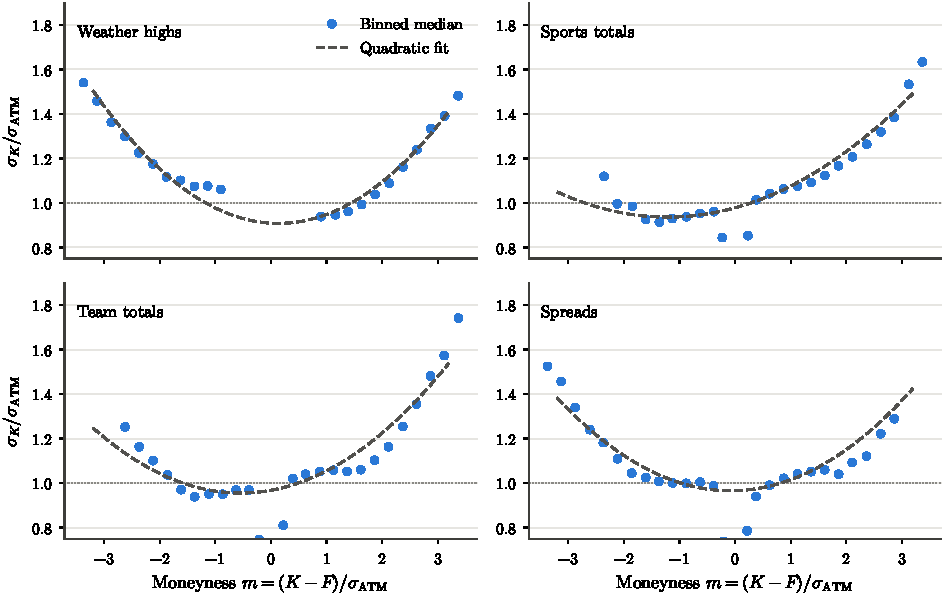
\includegraphics[width=\textwidth]{figures/fig_lad_smile.pdf}
\caption{Implied volatility smile. Median $\sigma_K/\satm$ in moneyness bins of width 0.25 (bins
with at least 30 strikes), all leads and both samples pooled, with the pooled quadratic fit of
\eqref{eq:lad-smile}. The dotted line is the flat smile of a normal implied distribution. Bins
near $m=0$ are noisy because $\sigma_K=(\Fmed-K)/\Phi^{-1}(S)$ has a small denominator there.}
\label{fig:lad-smile}
\end{figure}

The skew-$t$ summaries compare like with like (\cref{tab:lad-smile}, last four columns). The
implied skew has the right sign and roughly the right size. For sports totals the implied Bowley
skewness is 0.123 and 0.101 in the two samples, against 0.116 and 0.067 realised. Weather highs
are left-skewed in both the implied and the realised fits. Implied tails, however, are
consistently heavier than realised ones. The implied tail weight is 1.13--1.40 for sports and
1.23--1.29 for weather highs, against 1.03--1.19 and 1.04--1.05 realised. That gap is the
cross-strike form of the favourite--longshot bias~\citep{griffith1949,thalerziemba1988,snowbergwolfers2010}.

\subsubsection{Smile dynamics: sticky moneyness, not sticky strike}

\Cref{tab:lad-dyn} reports the regressions \eqref{eq:lad-atm}--\eqref{eq:lad-fixedk} on
consecutive snapshot pairs. Two pieces of evidence reject a sticky-strike smile.

\emph{The ATM point does not slide along the smile.} When the median moves, $\satm$ barely
responds. The slope $b$ is 0.017 for sports totals, $-0.031$ for team totals, $-0.020$ for spreads
and $-0.040$ for weather highs. A smile fixed in strike would give the pooled skew instead (0.065,
0.039, 0.013 and $-0.014$). Using each snapshot's own skew, the coefficient $\delta$ that should
equal 1 under sticky strike is between 0.06 and 0.54 in the weather and sports groups, and $\delta=1$ is rejected at $|t|\ge4.1$ for
totals, team totals and weather highs.

\emph{The volatility at a fixed strike moves with the median} (\cref{fig:lad-sticky}). With the
pooled smile, the sticky-moneyness coefficient $\gamma$ is 1.01 for spreads, 1.17 for weather highs,
1.31 for totals and 2.11 for team totals ($t$ from 9 to 25 against zero). Sticky strike ($\gamma=0$)
is rejected in every group. For totals and team totals the coefficient also exceeds one: the
smile moves more than one-for-one with the median, possibly because the wings re-price as the
game state changes.

The raw response has the sign sticky moneyness predicts. In sports totals, where $s>0$, the
volatility at a fixed strike falls when the median rises: $-0.081$ per unit of $\Delta\Fmed_n$
($t=-15.9$). With each snapshot's own smile the coefficients fall to 0.25--0.63 in sports,
consistent with attenuation from measurement error in snapshot-level $(s,c)$. Weather highs, whose
snapshot smiles are better determined, give 1.17 under either definition.
% source: summary.json:dynamics_atm, dynamics_fixed_strike

\begin{table}[t]
\centering\footnotesize
\setlength{\tabcolsep}{2.4pt}
\begin{threeparttable}
\caption{Smile dynamics between consecutive snapshots.}\label{tab:lad-dyn}
% source: summary.json:dynamics_atm and summary.json:dynamics_fixed_strike
\begin{tabular}{@{}lrccccccc@{}}
\toprule
 & & \multicolumn{2}{c}{ATM, \eqref{eq:lad-atm}} & \multicolumn{3}{c}{Fixed strike, \eqref{eq:lad-fixedk}} & \multicolumn{2}{c}{Backbone $\beta$} \\
\cmidrule(lr){3-4}\cmidrule(lr){5-7}\cmidrule(lr){8-9}
Group & Pairs & $b$ ($t$) & $\bar s$ & $\gamma$ pooled ($t_{\gamma=1}$) & $\gamma$ snapshot & $\partial\sigma_K/\partial\Fmed$ ($t$) & Within ($t$) & Cross ($t$) \\
\midrule
Weather highs & 4,230 & $-0.040$ ($-7.4$) & $-0.014$ & 1.17 (3.6) & 1.17 & 0.019 (2.0) & -- & -- \\
Sports totals & 3,984 & 0.017 (1.4) & 0.065 & 1.31 (4.5) & 0.63 & $-0.081$ ($-15.9$) & 0.28 (3.2) & 0.29 (13.2) \\
Team totals   & 2,566 & $-0.031$ ($-2.8$) & 0.039 & 2.11 (10.1) & 0.30 & $-0.117$ ($-14.1$) & $-0.12$ ($-2.9$) & 0.22 (13.8) \\
Spreads       & 2,250 & $-0.020$ ($-1.5$) & 0.013 & 1.01 (0.1) & 0.25 & $-0.003$ ($-0.4$) & -- & -- \\
Politics      & 155   & $-0.056$ ($-0.8$) & 0.017 & 0.68 ($-2.5$) & 0.33 & 0.055 (1.8) & 0.69 (1.2) & 0.20 (1.9) \\
\bottomrule
\end{tabular}
\begin{tablenotes}[flushleft]\footnotesize
\item Pairs of consecutive snapshots of one ladder, estimation sample (before 1 October 2026) and
holdout (October 2026) pooled. Fixed effects for each group and lead pair; $t$ clustered by event.
$b$: slope of $\Delta\satm/\satm$ on $\Delta\Fmed/\satm$. $\bar s$: mean pooled skew, the
sticky-strike prediction for $b$ (sticky moneyness predicts 0). The coefficient $\delta$ on
$s\,\Delta\Fmed/\satm$ with each snapshot's skew (1 under sticky strike) is 0.23, 0.06, 0.12, 0.54
and $-0.31$ in the five rows ($t_{\delta=1}=-4.9$, $-4.1$, $-5.3$, $-1.3$, $-6.4$). $\gamma$: coefficient
on the sticky-moneyness prediction $-(s+2cm)\Delta\Fmed/\satm$, using the group-and-lead pooled
smile or each snapshot's own smile (1 under sticky moneyness, 0 under sticky strike); the pooled
$\gamma$ has $t$ between 9.4 and 24.6 against zero (5.3 for politics). Fixed-strike pairs: 5,259
(weather highs), 28,108 (totals), 16,490 (team totals), 24,867 (spreads), 730 (politics).
$\partial\sigma_K/\partial\Fmed$: raw slope of the fixed-strike change on $\Delta\Fmed/\satm$.
Backbone: $\Delta\log\satm$ on $\Delta\log\Fmed$ within ladders, and $\log\satm$ on $\log\Fmed$
with series-by-lead fixed effects, for positive underlyings only.
\end{tablenotes}
\end{threeparttable}
\end{table}

\begin{figure}[t]
\centering
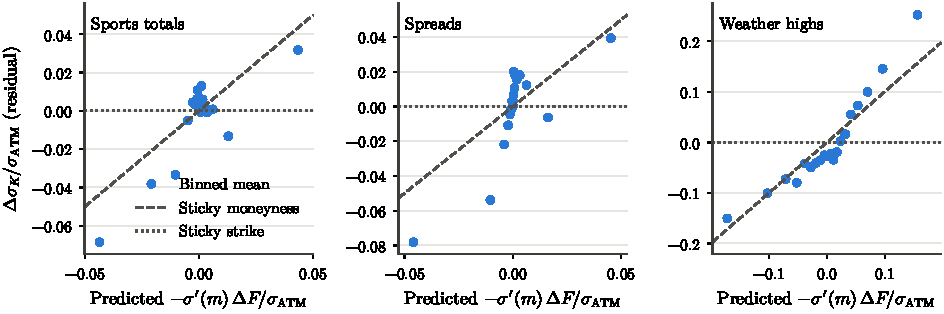
\includegraphics[width=\textwidth]{figures/fig_lad_sticky.pdf}
\caption{Fixed-strike volatility change against the sticky-moneyness prediction
$-\sigma'(m)\,\Delta\Fmed/\satm$ (pooled smile), after removing group-by-lead-pair means and
partialling out the level term of \eqref{eq:lad-fixedk}. Points are means in 20 quantile bins
of the prediction. Sticky moneyness predicts the dashed 45-degree line, sticky strike the dotted
zero line. In sports most pairs have small median moves; the slope is identified by the
larger moves.}
\label{fig:lad-sticky}
\end{figure}

\emph{Backbone.} For sports totals, $\satm$ rises with the level of the median both across games
($\beta=0.29$, $t=13.2$) and within a game between snapshots ($\beta=0.28$, $t=3.2$). Both are
well below the square-root exponent $\tfrac12$ of a Poisson count. For team totals the cross-section gives
$\beta=0.22$ but the within-game exponent is slightly negative ($-0.12$). The SABR-style level
backbone is therefore weak: the volatility of a ladder is set mainly by its moneyness and its
clock, not by the level of the underlying.

\subsubsection{ATM term structure}

\Cref{fig:lad-termstructure} plots $\log\satm$ against the lead within ladders. The estimated
exponents $\eta$ (\cref{tab:lad-term}) separate three information clocks.
% source: summary.json:term_structure
\begin{itemize}
\item \emph{Weather highs} have $\eta=0.773$ [0.760, 0.786], well above the uniform-clock value
  $\tfrac12$. Uncertainty about the daily maximum resolves late, during the afternoon of the
  measurement day.
\item \emph{Weather lows} have $\eta=0.480$ [0.413, 0.546], indistinguishable from $\tfrac12$.
  Their profile is flat from 16 to 8 hours, after the morning minimum has been observed.
\item \emph{Politics, entertainment and science} ladders are sub-diffusive (0.35, 0.19 and 0.24).
  Their information arrives in lumps close to resolution.
\item \emph{Sports ladders} have no pre-game time decay at all ($\eta=0.001$--$0.009$): nothing is
  learned about the score before the game starts.
\end{itemize}

\begin{figure}[t]
\centering
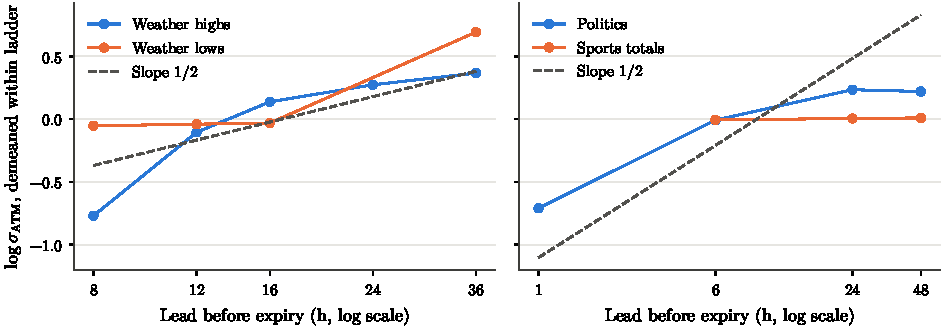
\includegraphics[width=\textwidth]{figures/fig_lad_termstructure.pdf}
\caption{ATM term structure. Mean of $\log\satm$, demeaned within ladder, by lead before expiry
(log scale). Left: weather highs and lows (hours before the measurement-day close). Right: politics and
sports totals (hours before the expected expiration; sports pre-game leads only). The dashed line
has slope $\tfrac12$, the uniform information clock.}
\label{fig:lad-termstructure}
\end{figure}

\subsubsection{Calibration against the realised outcome}

\Cref{tab:lad-calib} and \cref{fig:lad-calibration} test the implied distribution against
$X_T$. Sports ladders are calibrated in width and shape. In the holdout the width ratio is 1.02--1.03
(no $|t|$ above 1.1). The fractional PIT histogram is flat, with outer-decile shares of 0.192--0.202
against 0.2. In the \estim{} the widths are slightly too narrow (totals 1.045, $t=2.2$; spreads
1.144, $t=4.0$), and spreads put too much mass in the outer deciles (0.234); neither carries over
to the holdout.

Weather is too wide. The width ratio for highs is 0.941 ($t=-2.4$) and 0.890 ($t=-3.8$), and the
PIT puts too little mass in the outer deciles for both highs and lows (0.168--0.180, $t$ from
$-3.2$ to $-6.3$). Sports totals show a location bias: the realised total lands above the implied
median by $0.121\,\satm$ in the \estim{} ($t=5.1$) and $0.064\,\satm$ in the holdout ($t=2.4$).
% source: summary.json:width (lead_h = -1), summary.json:pit

The tail-mass comparison (\cref{fig:lad-calibration}, right; \cref{tab:lad-tails}) locates the
excess width in the wings.
\begin{itemize}
\item \emph{Weather highs.} Beyond $|m|\ge2.5$ the market prices 0.93--1.11\cents{} of tail mass
  per strike; realised frequencies are 0--0.30\cents{} ($z_{H_0}$ between $-0.5$ and $-2.6$, all
  negative).
\item \emph{Weather lows.} Every wing and threshold has $z_{H_0}<0$.
\item \emph{Sports.} The evidence is mixed. Holdout upper tails of totals at $|m|\ge2.5$ are
  overpriced (1.70\cents{} implied, 0.11\cents{} realised, $z_{H_0}=-2.2$), but the same cell in the
  \estim{} is not (1.77 against 2.19\cents).
\item \emph{Politics and entertainment.} Beyond $|m|\ge1.5$, wings are priced at 0.8--3.3\cents{} and
  are realised less often in most cells, but with at most 64 events per cell no $z_{H_0}$ is below
  $-1.3$.
\end{itemize}
% source: summary.json:tail_summary

\begin{table}[t]
\centering\small
\setlength{\tabcolsep}{4pt}
\begin{threeparttable}
\caption{Calibration of the implied distribution against the realised outcome.}\label{tab:lad-calib}
% source: summary.json:width (lead_h = -1) and summary.json:pit
\begin{tabular}{@{}lcccccc@{}}
\toprule
 & \multicolumn{2}{c}{Width ratio $\lambda$ ($t_{\lambda=1}$)} & \multicolumn{2}{c}{Location $\mu$ ($t$)} & \multicolumn{2}{c}{PIT outer-decile share ($t_{0.2}$)} \\
\cmidrule(lr){2-3}\cmidrule(lr){4-5}\cmidrule(lr){6-7}
Group & Estimation & Holdout & Estimation & Holdout & Estimation & Holdout \\
\midrule
Weather highs & 0.941 ($-2.4$) & 0.890 ($-3.8$) & 0.066 (1.9) & $-0.095$ ($-2.4$) & 0.178 ($-3.2$) & 0.170 ($-3.9$) \\
Weather lows  & 0.916 ($-0.7$) & 0.949 ($-0.7$) & $-0.081$ ($-1.5$) & 0.064 (0.8) & 0.168 ($-6.3$) & 0.180 ($-3.5$) \\
Sports totals & 1.045 (2.2) & 1.021 (1.0) & 0.121 (5.1) & 0.064 (2.4) & 0.196 ($-0.6$) & 0.192 ($-0.9$) \\
Team totals   & 1.045 (1.6) & 1.025 (1.0) & 0.127 (3.7) & 0.021 (0.6) & 0.199 ($-0.1$) & 0.202 (0.2) \\
Spreads       & 1.144 (4.0) & 1.027 (1.1) & 0.000 (0.0) & $-0.047$ ($-1.5$) & 0.234 (2.7) & 0.201 (0.1) \\
Politics      & 1.216 (1.0) & 1.297 (1.8) & $-0.152$ ($-0.9$) & 0.052 (0.3) & 0.192 ($-0.2$) & 0.233 (0.9) \\
Entertainment & 1.179 (1.9) & 0.852 ($-1.6$) & 0.013 (0.1) & 0.056 (0.3) & 0.205 (0.2) & 0.164 ($-2.8$) \\
\bottomrule
\end{tabular}
\begin{tablenotes}[flushleft]\footnotesize
\item One observation per snapshot, all leads pooled; estimation sample (before 1 October 2026),
holdout (October 2026). $\lambda$, $\mu$: interval-censored normal maximum likelihood for
$(X_T-\Fmed)/\satm$; $\lambda<1$ means the implied ATM width is too wide. PIT: fractional
histogram of the interval-censored probability integral transform; share of mass in the deciles
$[0,0.1)$ and $[0.9,1]$, 0.2 under calibration. All $t$ statistics cluster by event. Spread
locations are in the favourite's orientation.
\end{tablenotes}
\end{threeparttable}
\end{table}

\begin{figure}[t]
\centering
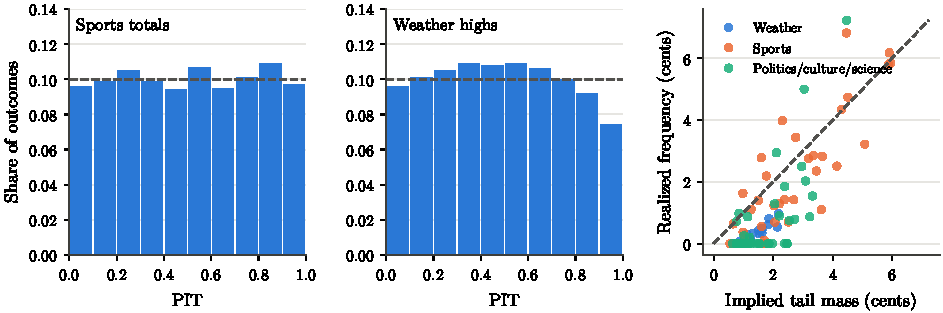
\includegraphics[width=\textwidth]{figures/fig_lad_calibration.pdf}
\caption{Calibration. Left and centre: fractional PIT histograms in the holdout (October 2026) for
sports totals and weather highs; the dashed line is the uniform density. Right: implied tail mass
against realised frequency, per group, sample, wing and threshold $|m|\ge1,\dots,2.5$ (thresholds
from 1.5 shown), in cents; the dashed line is calibration.}
\label{fig:lad-calibration}
\end{figure}

\subsubsection{Implied versus realised variance between snapshots}

\Cref{fig:lad-variance} and \cref{tab:lad-variance} report the ratio \eqref{eq:lad-vr}.
% source: summary.json:variance_between
\emph{Sports, pre-game.} Both terms are nearly zero, since neither the median nor the width moves,
and the ratio is not informative.
\emph{Sports, in play} (6 hours to 1 hour before expiry). Realised variance falls short of the
implied variance drop:
\begin{itemize}
\item totals 0.90 [0.81, 0.98];
\item spreads 0.92 [0.84, 1.04];
\item team totals 0.65 [0.59, 0.70].
\end{itemize}
The implied distribution narrows faster than its median moves: a variance premium, sizeable only
for team totals.

\emph{Weather highs} change sign across the day. The ratio is 1.02 from 36 to 24 hours, 0.66
[0.58, 0.73] overnight (24 to 16 hours) and 1.08 in the morning (16 to 12 hours). It reaches 1.55
[1.37, 1.74] in the afternoon (12 to 8 hours), when the median moves more than the narrowing of
the distribution allows. The weather median is also not a martingale. Its standardised drift is
$-0.046$ overnight ($t=-4.5$) and positive in the other three windows ($t$ from 2.8 to 5.8): the
market under-forecasts the daytime maximum until observations arrive.

\begin{figure}[t]
\centering
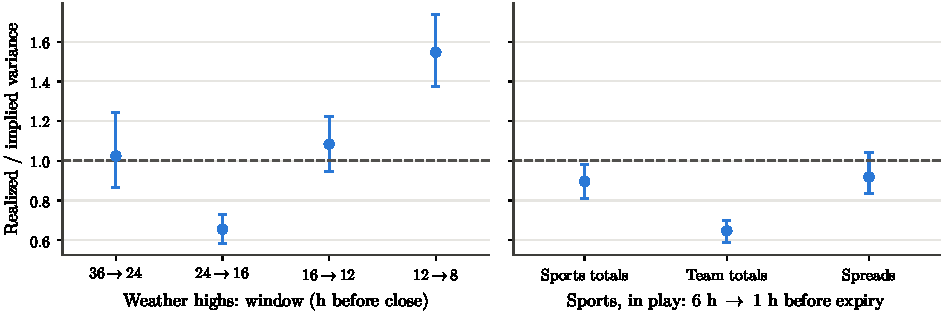
\includegraphics[width=\textwidth]{figures/fig_lad_variance.pdf}
\caption{Realised over implied variance between consecutive snapshots, \eqref{eq:lad-vr}, with
90\% cluster-bootstrap intervals over events. Left: weather highs by window (hours before the
measurement-day close). Right: sports ladders in play, 6 to 1 hours before the expected
expiration. The dashed line is equality.}
\label{fig:lad-variance}
\end{figure}

\subsubsection{Economic significance}

The wing premium is small in money terms.
% source: summary.json:pooled_rules (scope "all groups")
\begin{itemize}
\item \emph{Gating by model moneyness.} Selling the tail side of every leg with model moneyness
  $|m|\ge2.5$ at the snapshot quote, after the taker fee, returns $+0.23\cents$ per contract in the
  \estim{} ($t_{\text{risk}}=0.4$, 2,741 contracts) and $+1.10\cents$ in the holdout
  ($t_{\text{risk}}=2.0$, 3,006 contracts).
\item \emph{Gating by price alone.} The control (tail price at most 2\cents) returns $+0.31$ and
  $+0.25\cents$.
\item \emph{Within one price band.} Among tails priced at most 5\cents, legs with $|m|\ge2$ return
  $+0.29$ and $+0.49\cents$ while legs with $|m|<2$ return $-1.22$ and $-0.85\cents$: moneyness
  separates the overpriced wings from the rest.
\end{itemize}
The gain per contract is bounded by the 1\cents{} tick, and the evidence is weak once
settlement risk is taken into account. Net-of-fee arbitrage between legs (monotonicity or bracket
sums) appears in 30 of 24,192 snapshots. % source: summary.json:arbitrage (sums)

\subsubsection{Limitations}

Several limitations apply.
\begin{itemize}
\item \emph{Quotes.} They are hourly candle closes up to two hours old, without displayed size, and
  closes of different legs are not synchronous.
\item \emph{Spread filter.} The 5\cents{} filter discards many weather-low bracket sets and most
  far wings that have no bid.
\item \emph{Tick floor.} Wings quoted at the 1\cents{} tick inflate far-wing volatilities, so part of
  the measured curvature is a price-grid effect.
\item \emph{Interval censoring.} The realised outcome is known only up to the bracket containing
  it. This limits the precision of the realised skew-$t$ fits, which carry no intervals.
\item \emph{Fixed-strike coefficient.} With snapshot smiles it is attenuated by measurement error.
  With pooled smiles it inherits any misspecification of a common smile within a group and lead.
\item \emph{Sports clock.} The expected expiration of sports markets is a scheduled time, so the
  1 hour snapshot falls at different stages of different games.
\item \emph{Multiple comparisons.} We report many groups, leads and tests. The statements above
  rely on patterns that recur across groups or samples rather than on single cells.
\end{itemize}
